\section{Results of the registered gates}\label{sec:results}

\begin{table}[ht]
\centering\small
\begin{tabular}{@{}p{0.09\textwidth}p{0.075\textwidth}p{0.5\textwidth}p{0.2\textwidth}@{}}
\toprule
gate & grid & outcome (numbers from \texttt{summary.json}) & registered result \\ \midrule
D-a & $8\times8$ & above threshold, 10 seeds started at the closed form plus $10^{-3}$ noise (a stability check, not a basin test): relative $n$, $n_R$ and absolute $\omega$ deviations \DaWorstN{}, \DaWorstNR{}, \DaWorstOm{}; below: $\max|\psi|\le$ \DaBelowPsi{} & pass \\
D-b & $16\times16$ & eigenvalues of the solver's $768\times768$ finite-difference Jacobian matched one-to-one to the reference to \DbMatch{}; largest real part \DbMaxRe{} (the Goldstone mode). \emph{The registered sorted comparison gives $18.2$; see Section~\ref{sec:dd}} & pass with a replaced criterion \\
D-c & $16\times16$ & norm drift \DcNorm{}, energy drift \DcEnergy{} over $t=20$ (\DcSteps{} steps) & pass \\
D-d (i),(ii) & $8\times8$ & pump budget up to \DdBudgetMax{} (gate $10^{-8}$), stationarity residual up to \DdResidMax{} (gate $10^{-7}$); even $V_0=0$ gives \DdResidZero{} & \textbf{fail} \\
D-d (iii) & $8\times8$ & $\omega(V_0)-\omega(0)=$ \DdShiftA{}, \DdShiftB{}, \DdShiftC{} for $V_0=0.25,0.5,1$: between $0$ and $V_0$, increasing (medians at $t=4000$); in this box this is the area average of the gate, see text & pass (hypothesis; uninformative) \\
D-e & $16\times16$ & one step succeeds at $h=0.005,0.01,0.0125$ and returns an error at $0.02,0.05$ (threshold $0.01707$); no silent non-finite result; trajectory to $t=20$ within \DeTraj{} of CVODE & pass \\
D-f & $16\times16$ & error ratios \DfRatioA{} and \DfRatioB{} on halving $h$ (second order) & pass \\
D-g & $8\times8$ & planted bug: $n=$ \DgN{} instead of $10$; budget violated by $\ge$\DgBudget{} (\DgSeeds{} seeds, amendment A4) & pass \\
\bottomrule
\end{tabular}
\caption{Gates as registered. Every number is generated from the run records by \texttt{phase3\_paper\_numbers.py}.}
\end{table}

\begin{figure}[ht]
\centering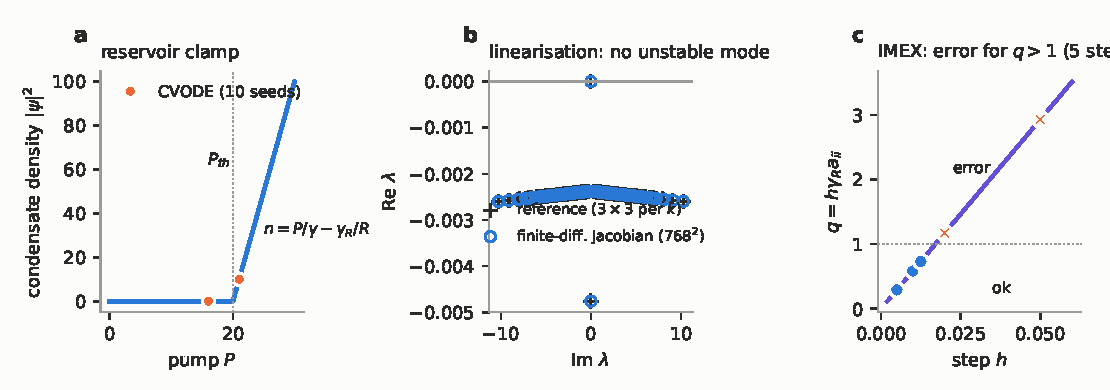
\includegraphics[width=\textwidth]{figs_exciton3/fig_solver.pdf}
\caption{Solver tests. (a) Steady-state density against pump: closed form (line) and ten CVODE runs per pump (dots; they
coincide to \DaWorstN{}). (b) The eigenvalues of a central-difference Jacobian of the solver's right-hand side (circles) lie on the reference spectrum
(crosses); the isolated points are the $k=0$ phase (Goldstone) and amplitude modes; the fast reservoir mode near $-\gamma_R$ is outside the plotted range. (c) The IMEX module's fixed-point stage:
contraction factor $q=h\gamma_Ra_{ii}$; it returns an error for $q=1.17$ and $2.93$ and succeeds for $q\leq0.73$ (the threshold $q=1$ is bracketed, not located).}
\end{figure}

\begin{failbox}
\textbf{The registered gate-sweep gates failed.} At $t=4000$ the stationarity residual of the gated states is up to \DdResidMax{}
and the pump budget is violated by up to \DdBudgetMax{}, against thresholds $10^{-7}$ and $10^{-8}$; the ungated state also
exceeds its threshold (\DdResidZero{}). The horizon was set from the decay rate of the ungated Bogoliubov modes ($2.4\times10^{-3}$) applied to a $10^{-3}$ perturbation;
the gated states start $O(0.1)$ from the uniform state and the slowest linear decay rates about them are $1.4$--$2.1\times10^{-3}$
(reviewer's linearisation), so $e^{-1.4\times10^{-3}\cdot4000}\approx3\times10^{-3}$ of an $O(0.1)$ amplitude is left. The ungated failure
($1.6\times10^{-7}$) was predictable from the registered numbers. All ten seeds end on the same state to all printed digits, and the
residual does not depend on the integrator tolerance ($\mathrm{rtol}=10^{-8}$ to $10^{-12}$ give \ExplRtolResid{}), so it is not
integration error. \emph{Exploratory} continuations (not gates, one seed each) to $t=16000$ give residual \ExplResid{} and budget
violation \ExplBudget{} for $V_0=0.5$, which would pass; \ExplOtherSentence{}
\end{failbox}

\begin{figure}[ht]
\centering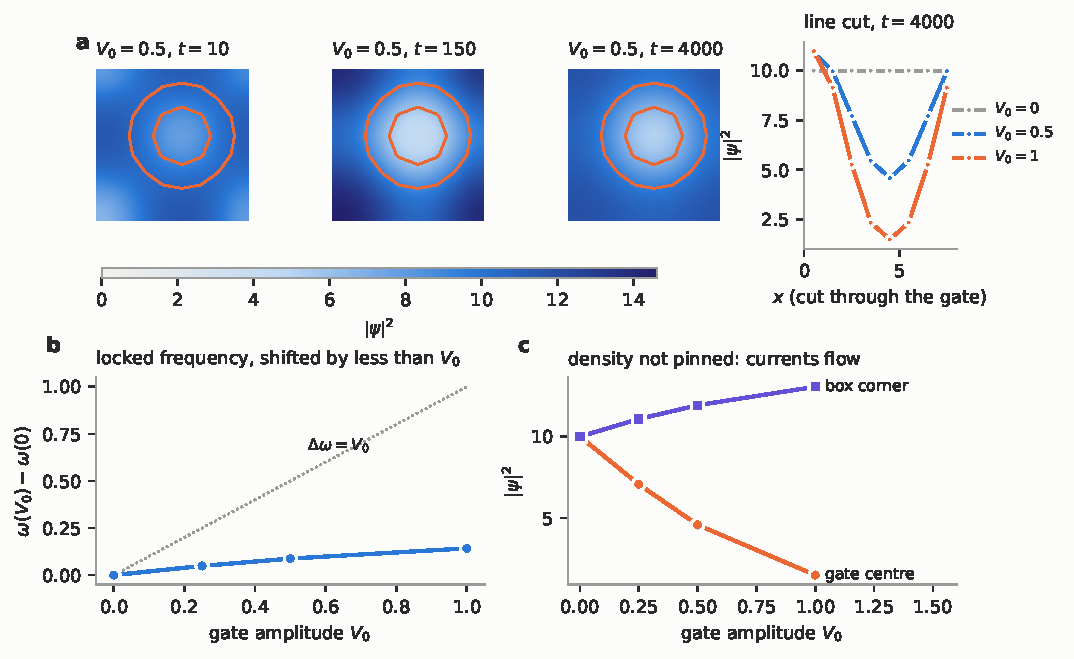
\includegraphics[width=\textwidth]{figs_exciton3/fig_gate.pdf}
\caption{A gated driven-dissipative condensate on the $8\times8$ grid ($\sigma=1.5$), uniform pump $P=21$.
(a) Density from the uniform start with noise at three times (orange: contours of the gate; fields are
bicubic interpolations of the $8\times8$ values) and a line cut through the gate at $t=4000$ for three amplitudes.
(b) The locked emission frequency shifts with the gate amplitude by less than $V_0$; in this small box that is the area average of the gate (text).
(c) Density at the gate centre falls and at the box corner rises: the density is \emph{not} pinned at its ungated value,
because the single locked frequency requires currents (largest current density
\DdJA{}--\DdJB{} for $V_0=0.25$--$0.5$).}
\end{figure}

\paragraph{What the gate sweep shows, and does not show.} In the small box the gate depletes the condensate at its centre
(from $10$ to \DdCentreA{}, \DdCentreB{}, \DdCentreC{} for $V_0=0.25,0.5,1$, while the corner rises to \DdCornerA{}, \DdCornerB{},
\DdCornerC{}), and currents flow. The single emission frequency moves by \DdShiftA{}, \DdShiftB{}, \DdShiftC{}.
\emph{That shift is a box-size artefact and carries little information.} An independent re-solution of the same stationary states by the
reviewer (own Newton solver; it reproduces the shifts to five digits) at fixed gate width $\sigma=1.5$ gives, for $V_0=1$,
$0.142$ ($L=8$), $0.024$ ($L=16$), $0.0055$ ($L=32$): $\Delta\omega$ falls like $L^{-2}$ and at small $V_0$ equals the area average
of the gate, $V_0\,2\pi\sigma^2/L^2$. ``Between $0$ and $V_0$'' is therefore implied by any bounded non-negative potential averaged
over a periodic box, and hypothesis (iii) of D-d, though it passed, does not test the model. Nor is the $8\times8$, $\sigma=1.5$
problem equivalent to the registered $16\times16$, $\sigma=3$ one at ``the same $\sigma/L$'': the reviewer's solution for the registered
geometry gives shifts $0.046,0.077,0.107$ and central densities $5.8,2.4,0.10$ for $V_0=0.25,0.5,1$, against $0.049,0.088,0.142$ and
$7.1,4.6,1.5$ here, and its slowest mode at $V_0=1$ is about $3\times10^{-4}$, so the registered horizon would have failed there far
worse. The linearisation about the numerical states has no unstable mode within the (relaxation-limited) accuracy \DdMaxReLambda{}.
No finite-size study of our own was made, and the dependence on the gate width and on the pump was not scanned.

\paragraph{The ARKode-style module.} It does what its design says: a fixed-point implicit stage that converges iff
$h\gamma_Ra_{ii}<1$, so for the stiff reservoir of this model ($\gamma_R=200$) the step is limited to $0.017$ while CVODE's BDF
takes the steps it chooses; with $h$ below the threshold it is second order and agrees with CVODE to \DeTraj{}. It is not
an adaptive stiff integrator and the library's default \texttt{ImexSolver} should not be used for stiff problems without the
replacement of the implicit stage.

\paragraph{Cost.} The pinned CVODE factorises a dense matrix every few steps (43 ms per step at 768 unknowns, 1.4 s per
$t=20$ at 192 unknowns); this, not the physics, set the grid of D-d. A matrix-free Krylov implicit solver (the spectral Laplacian makes the Jacobian dense, so banded storage does not apply), or an
exponential or split treatment of the linear kinetic term, is the obvious requirement for a $64\times64$ grid and was not
available in the pinned tree.
